% !TeX root = ./Tuneable_Lasers.tex

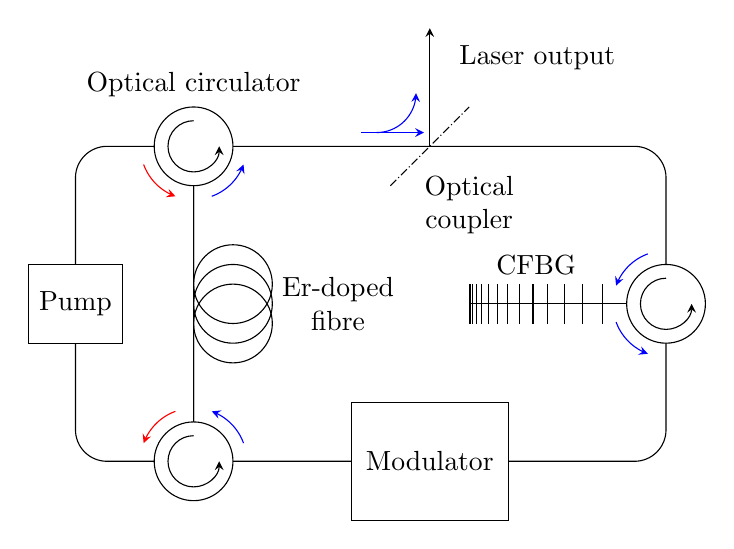
\begin{tikzpicture}
% Two laser loops
\draw [rounded corners=4mm] (0,0) rectangle ++(6,4);
\draw [rounded corners=4mm] (0,0) rectangle ++(-1.5,4);

% Gain
\draw (0.5,2.25) circle (0.5cm);
\draw (0.5,2) circle (0.5cm) node [anchor=west,xshift=0.5cm,align=center] {Er-doped \\ fibre};
\draw (0.5,1.75) circle (0.5cm);

% Modulator and pump
\filldraw[fill=white, draw=black] (2,-0.75) rectangle ++(2,1.5) node [midway] {Modulator};
\filldraw[fill=white, draw=black] (-2.1,1.5) rectangle ++(1.2,1) node [midway] {Pump};

% Coupler and output
\draw[-stealth] (3,4) -- (3,5.5) node [pos=0.75,anchor=west,xshift=0.25cm] {Laser output};
\draw[densely dashdotted] (2.5,3.5) -- (3.5,4.5) node [pos=1,anchor=north,yshift=-0.75cm,align=center] {Optical \\ coupler};

% Circulators
\filldraw[fill=white, draw=black] (6,2) circle (0.5cm);
\draw[->,>=stealth] (6,2.325) arc (90:360:0.325cm);

\filldraw[fill=white, draw=black] (0,0) circle (0.5cm);
\draw[->,>=stealth] (0,0.325) arc (90:360:0.325cm);

\filldraw[fill=white, draw=black] (0,4) circle (0.5cm) node [anchor=south,align=center,yshift=0.5cm] {Optical circulator};
\draw[->,>=stealth] (0,4.325) arc (90:360:0.325cm);

% Arrows
\draw [->,>=stealth,domain=20:70,blue] plot ({0.675*cos(\x)}, {0.675*sin(\x)});
\draw [->,>=stealth,domain=110:160,red] plot ({0.675*cos(\x)}, {0.675*sin(\x)});
\draw [->,>=stealth,domain=110:160,blue] plot ({6+0.675*cos(\x)}, {2+0.675*sin(\x)});
\draw [->,>=stealth,domain=200:250,blue] plot ({6+0.675*cos(\x)}, {2+0.675*sin(\x)});
\draw [->,>=stealth,domain=200:250,red] plot ({0.675*cos(\x)}, {4+0.675*sin(\x)});
\draw [->,>=stealth,domain=290:340,blue] plot ({0.675*cos(\x)}, {4+0.675*sin(\x)});

\draw [->,>=stealth,domain=270:360,blue] plot ({2.325+0.5*cos(\x)}, {4.675+0.5*sin(\x)});
\draw [->,>=stealth,blue] (2.125, 4.675-0.5) -- (2.325+0.6, 4.675-0.5);

% Grating
\draw (5.5,2) -- (3.5,2) node [pos=0.5,anchor=south,yshift=0.25cm,xshift=-0.15cm] {CFBG};
\foreach \i in {0,...,13}
	\draw (3.5 + \i*\i/100,1.75) -- (3.5 + \i*\i/100,2.25);

\end{tikzpicture}